% \chapter{Задания} 
\chapter{Эксперимент 1: Исследование расслоения динамической памяти}

\section{Цель эксперимента}
Определить способ трансляции физического адреса, используемый при обращении к динамической памяти.  

\section{Описание проблемы}
В связи с конструктивной неоднородностью оперативной памяти, обращение к последовательно расположенным данным требует различного времени. В связи с этим, для создания эффективных программ необходимо учитывать расслоение памяти, характеризуемое способом трансляции физического адреса. 

\section{Суть эксперимента}
Для определения способа трансляции физического адреса при формировании сигналов выборки банка, выборки строки и столбца запоминающего массива применяется процедура замера времени обращения к динамической памяти по последовательным адресам с изменяющимся шагом чтения. Для сравнения времен используется обращение к одинаковому количеству различных ячеек,  отстоящих друг от друга  на  определенный шаг. Результат эксперимента представляется зависимостью  времени (или количества тактов процессора), потраченного на чтение ячеек от шага чтения. 

\section{Условия эксперимента}
\begin{enumerate}
    \item Единицы измерения по Ох - Байты;
    \item Единицы измерения по Оу - Такты;
    \item Максимальное расстояние между читаемыми данными: \textbf{32};
    \item Шаг увеличения расстояния между читаемыми 4-х байтовыми ячейками: \textbf{64};
    \item Размер массива: \textbf{8};
\end{enumerate}

\section{Результаты эксперимента}
\begin{figure}[ht!]
    \centering
    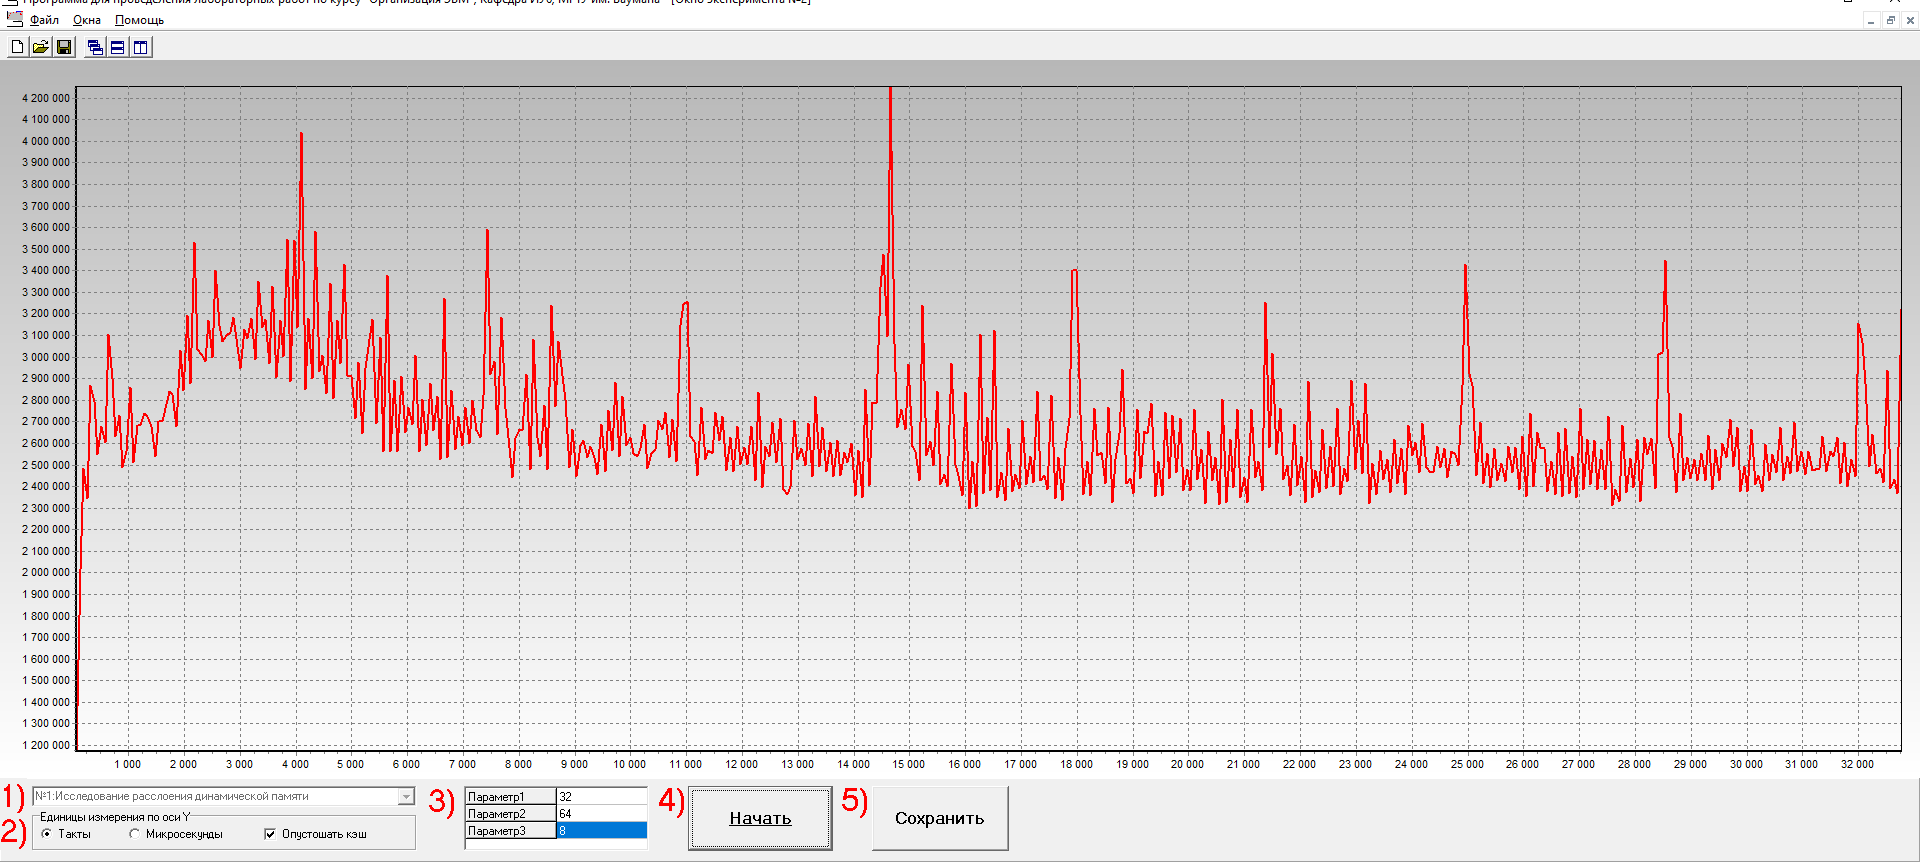
\includegraphics[width=170mm]{./img/1.png}
    \caption{Эксперимент 1: Исследование расслоения динамической памяти\label{overflow1}}
\end{figure}

\section{Вывод}
При работе с оперативной памятью следует учитывать, что её доступ к последовательно расположенным данным может занимать разное время из-за неоднородности. 
При разработке программ необходимо обращать внимание на эту особенность и оптимизировать обработку данных, учитывая расслоение памяти.